\documentclass[10pt,a4paper]{article}
\usepackage[a4paper]{geometry}

\usepackage[utf8x]{inputenc}
\usepackage{polski}

\usepackage{amsmath}
\usepackage{amssymb}
\usepackage{amsthm}

\usepackage{graphicx}
\usepackage{sidecap}

\usepackage{tikz}
\usetikzlibrary{trees}

\theoremstyle{plain}
\newtheorem{theorem}{Twierdzenie}
\newtheorem{lemma}{Lemat}
\theoremstyle{definition}
\newtheorem*{definition}{Definicja}
\newtheorem*{example}{Przykład}
\newtheorem*{remark}{Uwaga}

\newcommand{\impl}{\rightarrow}
\newcommand{\N}{\mathbb{N}}

\newcommand{\header}[1]{\noindent\textbf{#1}}

\title{Teoria Programowanie w Logice}
\author{}
\date{Semestr letni 2013}

\begin{document}
\maketitle

\section{Dowody Hilberta i twierdzenie Posta o pełności}

\header{Język:}

\begin{itemize}
  \item przeliczalnie wiele zmiennych: $\{x_i\}_{i\in\N}$;
  \item funktory: $\impl, \neg$;
  \item zbiór formuł sensownych $S$: najmniejszy zbiór, taki że:
  \begin{enumerate}
    \item $\{x_i\} \subset S$;
    \item jeśli $A, B \in S$, to $A \impl B \in S$ i $\neg A \in S$.
  \end{enumerate}
\end{itemize}

\begin{definition}
$D \subset S$ jest zamknięty na Modus Ponens (MP), gdy
$$\text{jeśli } A \impl B \in D \text{ i } A \in D \text{, to } B \in D.$$
\end{definition}

\begin{lemma}
Jeśli $\alpha$ to pewna rodzina zbiorów zamkniętych na MP,
to $\bigcap\alpha$ jest zamknięty na MP.
\end{lemma}

\begin{lemma}
Jeśli $\alpha$ to pewna rodzina zbiorów zamkniętych na MP, która jest łańcuchem,
to $\bigcup\alpha$ jest zamknięty na MP.
\end{lemma}

\begin{lemma}
Dla każdego $X \subset S$ istnieje najmniejszy zbiór $Y$, taki że
\begin{enumerate}
  \item $X \subset Y$;
  \item $Y$ jest zamknięty na MP.
\end{enumerate}
\end{lemma}

\begin{proof}
$Y = \bigcap \{
  Z \subset S : X \subset Z \text{ i } Z \text { zamknięty na MP}
\}.$
\end{proof}

Taki $Y$ nazywamy \emph{konsekwencją} $X$. ($Cn: 2^S \ni X \mapsto Y \in 2^S$)

\bigskip

\header{Fakty o $Cn$}

\begin{enumerate}
  \item Jeśli $X$ jest zamknięty na MP, to $Cn(X) = X$.
  \item $X \subset Cn(X)$.
  \item Jeśli $X \subset Y$, to $Cn(X) \subset Cn(Y)$.
  \item $Cn(Cn(X)) = Cn(X)$.
  \item $Cn(X) = \bigcup\{
    Cn(Y) : Y \subset X \text{ i } X \text{ jest skończony}
  \}$.
    \begin{proof}
      $\supset$ -- trywialny. $\subset$ -- Wystarczy pokazać, że prawa strona
      jest zamknięta na MP. $A \impl B \in \bigcup \{ \ldots \}$, więc
      $A \impl B \in Cn(Y_1)$, $A \in \bigcup \{ \ldots \}$, więc
      $A \in Cn(Y_2)$, zatem $B \in Cn(Y_1 \cup Y_2)$.
      Na koniec zauważamy, że $Y_1 \cup Y_2$ jest skończonym podzbiorem $X$.
    \end{proof}
  \item $Cn(\emptyset) = \emptyset$.
\end{enumerate}

\bigskip

\header{Alternatywne opisy $Cn$}
\begin{align*}
& H^i: 2^S \to 2^S\\
& H^0(X) = X\\
& H^{n+1}(X) = H^n(X) \cup \{
    B \in S : \exists_{A \in S} (A \impl B \in H^n(X) \text{ i } A \in H^n(X))
  \}\\
& H(X) = \bigcup_{n = 0}^\infty H^n(X)
\end{align*}

\begin{lemma}
$Cn(X) = H(X).$
\end{lemma}

\begin{proof}
$\subset$ -- łatwy, $\supset$ -- przez indukcję ze względu na $n$.
\end{proof}

\begin{definition}[Dowód Hilberta]
$A \in S$ ma dowód Hilberta ze zbioru formuł $X$, gdy istnieje skończony ciąg
formuł $A_0, A_1, \ldots, A_n$, taki że $A_n = A$ i dla każdego $i$:
\begin{itemize}
  \item $A_i \in X$ lub
  \item istnieją $A_j, A_k$, takie że $j, k < i$ i $A_j = A_k \impl A_i$.
\end{itemize}
\end{definition}

%TODO: tu by można jeszcze wspomnieć o drzewowej reprezentacji dowodu.

\begin{definition}[Konsewkencja dowodowa]
$Cn^*(X) := \{ A \in S: A \text{ ma dowód z } X\}$
\end{definition}

\begin{lemma}
$Cn(X) = Cn^*(X)$
\end{lemma}

\begin{proof}
$\supset$ -- przez indukcję ze względu na długość dowodu,
$\subset$ -- przez sklejenie dowodów Hilberta.
%TODO: tę drugą część można by rozpisać dokładniej.
\end{proof}

\bigskip

\begin{definition}[Logika klasyczna]
Niech $L \subset S$ będzie najmniejszym zbiorem zawierającym (dla dowolnych
$A, B, C \in S$)
\begin{itemize}
  \item $K: A \impl (B \impl A)$
  \item $S: (A \impl (B \impl C)) \impl ((A \impl B) \impl (A \impl C))$
  \item $N: (\neg A \impl \neg B) \impl ((\neg A \impl B) \impl A)$
\end{itemize}
oraz zamkniętym na MP.
\end{definition}

\begin{example}
$I: A \impl A \in L$, ponieważ:
\begin{itemize}
  \item $(A \impl (B \impl A)) \impl ((A \impl B) \impl (A \impl A))$
    \quad(aksjomat $S$)
  \item $A \impl (B \impl A)$ \quad(aksjomat $K$)
  \item $(A \impl B) \impl (A \impl A)$ \quad(Modus Ponens)
  \item $(A \impl (C \impl A)) \impl (A \impl A)$ \quad($B := C \impl A$)
  \item $A \impl (C \impl A)$ \quad(aksjomat $K$)
  \item $A \impl A$ \quad(Modus Ponens)
\end{itemize}
\end{example}

\noindent Notacja: $Cn_L(X) := C_n(L \cup X)$.

\begin{theorem}[O dedukcji wprost, TDW]
$b \in Cn_L(X \cup \{a\})$ wtedy i tylko wtedy, gdy $a \impl b \in Cn_L(X)$.
\end{theorem}

\begin{proof}
$\Leftarrow$ -- trywialny. $\Rightarrow$ -- przez indukcję ze względu
na długość dowodu $b$.  %TODO: napisać tę drugą część.
\end{proof}

\begin{theorem}[O dedukcji nie wprost, TDN]
Jeśli $z, \neg z \in Cn_L(X \cup \{a, \neg b\})$, to $a \impl b \in Cn_L(X)$.
\end{theorem}

\begin{proof}
\begin{flalign*}
\neg b \impl z &\in Cn_L(X \cup \{a\}) && \text{z TDW}\\
\neg b \impl \neg z &\in Cn_L(X \cup \{a\}) && \text{z TDW}\\
(\neg b \impl \neg z) \impl ((\neg b \impl z) \impl b) 
  &\in L \subset Cn_L(X \cup\{a\}) && \text{aksjomat N}\\
b &\in Cn_L(X \cup \{a\}) && \text{MP} \times 2\\
a \impl b &\in Cn_L(X) && \text{TDW}
\end{flalign*}
\end{proof}

\begin{theorem}
Jeśli $L' \subset S$ jest zbiorem zamkniętym na MP, w którym prawdziwe jest TDW,
to $K, S \in L'$.
\end{theorem}

\begin{proof}
 ~\begin{itemize}
    \item $K \in L'$:
      \begin{flalign*}
        a &\in Cn_{L'}(\{a\} \cup \{b\}) && \\
        b \impl a &\in Cn_{L'}(\{a\}) && \text{z TDW} \\
        a \impl (b \impl a) &\in Cn_{L'}(\emptyset) = L' && \text{z TDW}
      \end{flalign*}
    \item $S \in L'$:
      \begin{flalign*}
        a &\in Cn_{L'}(\{a\impl (b\impl c), a \impl b, a\}) && \\
        b &\in Cn_{L'}(\{a\impl (b\impl c), a \impl b, a\}) &&
        \text{MP na }a\impl b\text{ i }a \\
        b \impl c &\in Cn_{L'}(\{a\impl (b\impl c), a \impl b, a\}) &&
        \text{MP na }a\impl (b \impl c)\text{ i }a \\
        c &\in Cn_{L'}(\{a\impl (b\impl c), a \impl b, a\}) &&
        \text{MP na }b \impl c\text{ i }b \\
        (a \impl c) &\in Cn_{L'}(\{a\impl (b\impl c), a \impl b\}) &&
        \text{z TDW} \\
        (a\impl b) \impl (a \impl c) &\in Cn_{L'}(\{a\impl (b\impl c)\}) &&
        \text{z TDW} \\
        (a\impl (b\impl c)) \impl ((a\impl b) \impl (a \impl c)) &\in
        Cn_{L'}(\emptyset) = L' && \text{z TDW} 
      \end{flalign*}
  \end{itemize}
\end{proof}

\begin{theorem}
Jeśli $L' \subset S$ jest zbiorem zamkniętym na MP, w którym prawdziwe jest TDN,
to $K, S, N \in L'$.
\end{theorem}

\begin{proof}
  ~\begin{itemize}
    \item W~$L'$ zachodzi TDW (zatem $K, S \in L'$):
      \begin{itemize}
        \item W każdym zbiorze zamkniętym na MP zachodzi:
          jeśli $b \impl a \in Cn_{L'}(X)$, to $a \in Cn_{L'}(X\cup\{b\})$.
        \item Implikacja w drugą stronę (jeśli $a \in Cn_{L'}(X\cup\{b\})$,
            to $b \impl a \in Cn_{L'}(X)$) zachodzi, bo:
          \begin{flalign*}
            a &\in Cn_{L'}(X\cup\{b\}) \subset Cn_{L'}(X\cup\{b,\neg a\})
            && \text{z założenia} \\
            \neg a &\in Cn_{L'}(X\cup\{b,\neg a\}) && \\
            b \impl a &\in Cn_{L'}(X) && \text{z TDN}
          \end{flalign*}
      \end{itemize}
    \item $N \in L'$:
      \begin{flalign*}
        \neg b, b &\in Cn_{L'}(\{\neg a \impl \neg b,\neg a \impl b, \neg a\})
        && \text{dwa razy MP} \\
        (\neg a \impl b) \impl a &\in Cn_{L'}(\{\neg a \impl \neg b\})
        && \text{z TDN} \\
        (\neg a \impl \neg b) \impl ((\neg a \impl b) \impl a)
        &\in Cn_{L'}(\emptyset) && \text{z TDW}
      \end{flalign*}
  \end{itemize}
\end{proof}

\header{Konstrukcje drzewowe dowodów}

\begin{figure}[h]
\caption{Drzewo Modus Ponens}
\centering 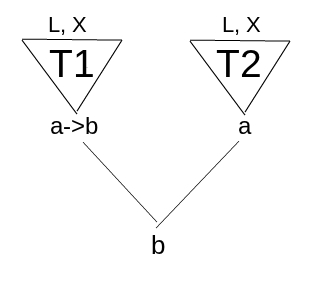
\includegraphics[width=0.3\textwidth]{img/drzewoMP}
\end{figure}

\begin{figure}[h]
\caption{TDW jako transformacja drzewa dowodu}
\centering 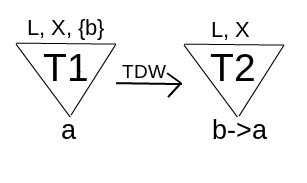
\includegraphics[width=0.4\textwidth]{img/drzewoTDW}
\end{figure}

Baza indukcji konstrukcji drzewa TDW:
\begin{itemize}
\item T1 jest punktem $a \in L \cup X$, robię $(K_{a, b}$ and $a) 
\Rightarrow b \rightarrow a$
\item T1 jest punktem $b$, robię $((S$ and $K)$ and $K) 
\Rightarrow b \rightarrow b$
\end{itemize}

\begin{figure}[h]
\caption{Indukcyjna konstrukcja drzewa TDW}
\centering 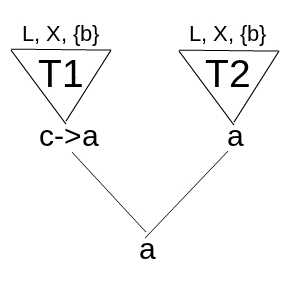
\includegraphics[width=0.25\textwidth]{img/drzewoMP2}
\centering 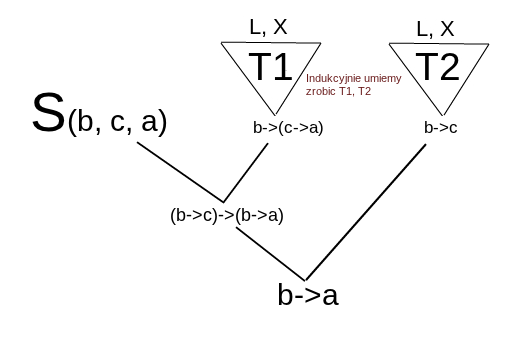
\includegraphics[width=0.5\textwidth]{img/drzewoTDWindukcyjnie}

\caption{Indukcyjna konstrukcja drzewa TDN}
\centering 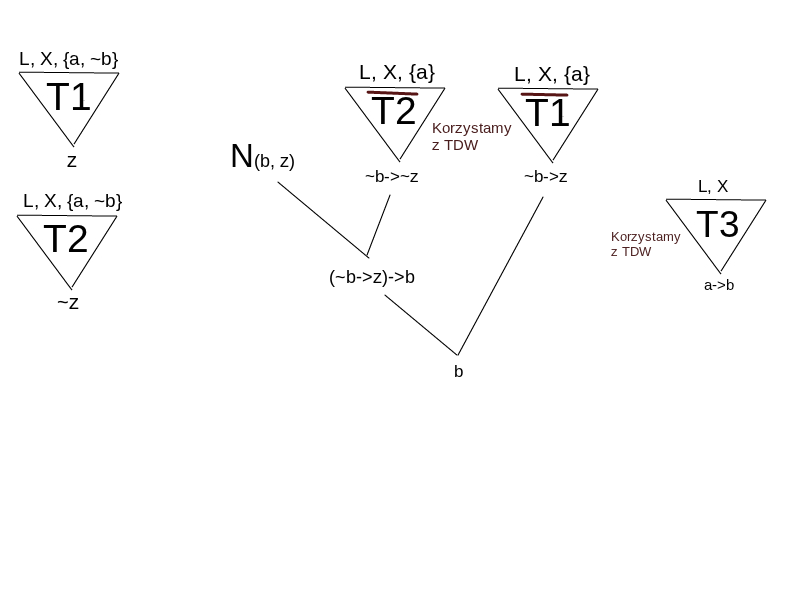
\includegraphics[width=0.7\textwidth]{img/drzewoTDN}
\end{figure}


\header{Ćwiczenia}

\begin{enumerate}
  \item $\neg \neg p \impl p \in L$.
      \quad Dowód: TDN dla $Cn_{L}(\{\neg \neg p, \neg p\})$.
  \item $p \impl \neg \neg p \in L$.
      \quad Dowód: 1. i TDN dla $Cn_{L}(\{p, \neg \neg \neg p\})$.
  \item $(p \impl q) \impl ((q \impl r) 
      \impl (p \impl r)) \in L$.
      \quad Dowód: TDW dla $Cn_{L}(\{p \impl q, q \impl r, p\})$.
  \item $(p \impl q) \impl (\neg q \impl \neg p) \in L$.
      \quad Dowód: TDN dla $Cn_{L}(\{p \impl q, \neg q, \neg \neg p\})$.
  \item Prawo wyłączonego środka:
      $(p \impl q) \impl ((\neg p \impl q) \impl q) \in L$.
    \begin{proof}
      \begin{flalign*}
        \neg q &\in Cn_{L}(\{p \impl q, \neg p \impl q, \neg q\}) &&\\
        \neg q \impl \neg p &\in Cn_{L}(\{p \impl q, \neg p \impl q, \neg q\})
            && \text{ćw. 4} \\
        \neg p &\in Cn_{L}(\{p \impl q, \neg p \impl q, \neg q\})
            && \text{MP} \\
        q &\in Cn_{L}(\{p \impl q, \neg p \impl q, \neg q\}) && \text{MP} \\
        (\neg p \impl q) \impl q &\in Cn_{L}(\{p \impl q\}) && \text{TDN} \\
        (p \impl q) \impl ((\neg p \impl q) \impl q) &\in Cn_{L}(\emptyset) = L
            && \text{TDW}
      \end{flalign*}
    \end{proof}
  \item Prawo Pierce'a: $((p \impl q) \impl p) \impl p \in L$.
    \begin{proof}
      \begin{flalign*}
        \neg p \impl (\neg q \impl \neg p) 
            &\in Cn_L(\{(p \impl q) \impl p, \neg p\}) && \text{aksjomat } S\\
        \neg q \impl \neg p &\in Cn_{L}(\cdots) && \text{MP}\\
        p \impl q &\in Cn_{L}(\cdots) && \text{ćw. 4}\\
        p &\in Cn_{L}(\cdots) && \text{MP}\\
        \neg p &\in Cn_{L}(\cdots) && \\
        ((p \impl q) \impl p) \impl p &\in Cn_{L}(\emptyset) = L && \text{TDN}
      \end{flalign*}
    \end{proof}
\end{enumerate}

\begin{remark}
  Pomimo że prawo Pierce'a da się wyrazić bez użycia negacji,
  \emph{nie należy ono} do logiki intuicjonistycznej (tzn.
  nie da się go wyprowadzić używając jedynie $K$ i~$S$).
\end{remark}

\begin{definition}
Zbiór $X \subset S$ jest sprzeczny, gdy $Cn_L(X) = S$.
\end{definition}

\begin{definition}
Zbiór $X \subset S$ jest zupełny, gdy 
$\forall_{a \in S} a \in S \text{ lub } \neg a \in S$.
\end{definition}

\begin{theorem}[Twierdzenie Lindenbauma]
Dowolny niesprzeczny zbiór $X \subset S$ może być rozszerzony do zbioru
$Y \supset X$, który jest zamknięty na MP, niesprzeczny i zupełny.
\end{theorem}

\begin{proof}[Dowód kreatywny]
Formuły to skończone napisy nad przeliczalnym alfabetem, zatem jest ich
przeliczalnie wiele. Możemy więc ustawić je w ciąg $s_0, s_1, \ldots$. 
Rozważmy ciąg $Y_i$, taki że $Y_0 = Cn_L(X)$ oraz

$$Y_{n+1} = \begin{cases}
  Cn_L(Y_n \cup \{s_n\}) & 
    \text{jeśli } Y_n \cup \{s_n\} \text{ jest niesprzeczny}\\
  Y_n & \text{wpp.}
\end{cases}$$

Niech $Y = \bigcup_{i\in\N} Y_i$. Wystarczy wykazać, że $Y$ ma własności
przedstawione w tezie.

Z definicji wynika, że zbiory $Y_i$ są zamknięte na MP, niesprzeczne 
i tworzą łańcuch. Łatwo można wykazać, że w takim razie również ich
suma jest zamknięta na MP i niesprzeczna.

Zupełność wymaga nieco więcej uwagi. Dowód przeprowadzimy nie wprost.
Załóżmy, że istnieje formuła $a$ taka, że $a, \neg a \not \in Y$.
Niech $a = s_i$ oraz $\neg a = s_j$. Skoro $a \not \in Y$, to
w szczególności $a \not \in Y_{i+1}$, zatem z definicji $Y_i \cup \{a\}$
jest sprzeczny. Analogicznie $Y_j \cup \{\neg a\}$ jest sprzeczny.
Oznaczmy $k=\max(i, j)$. Wtedy $Y_i,Y_j \subset Y_k$ i z monotoniczności
konsekwencji mamy, że $Cn_L(Y_k \cup \{a\}) = Cn_L(Y_k \cup \{\neg a\}) = S$.

Weźmy dowolną formułę $b \in S$. Z TDW mamy, że
$a \impl b, \neg a \impl b \in Cn_L(Y_k)$. Stosując prawo wyłączonego środka
możemy wykazać, że $b \in Y_k$. Skoro jednak $b$ było dowolną formułą, to
$Y_k = S$, co prowadzi do sprzeczności z faktem, że zbiory $Y_i$ są
niesprzeczne.
\end{proof}

\begin{proof}[Dowód bezmyślny]Z lematu Kuratowskiego-Zorna.\end{proof}

\begin{theorem}[Relatywne twierdzenie Lindenbauma]

Dla każdego zbioru $X \subset S$, takiego że $X = Cn_L(X)$, oraz każdej
formuły $a \not \in X$ istnieje zbiór $Y \subset S$, taki że
\begin{itemize}
  \item $Y \supset X$,
  \item $Y$ jest zamknięty na MP,
  \item $a \not \in Y$,
  \item $\forall_{b \not \in Y} a \in Cn_L(Y \cup \{b\})$ 
    ($Y$ nie da się już rozszerzyć zachowując powyższe warunki).
\end{itemize}
\end{theorem}

\begin{proof}Jak wyżej.\end{proof}

\begin{definition}
Matrycą logiczną nazywamy czwórkę $M=(U, U^*, f^\impl, f^\neg)$, taką że
\begin{itemize}
  \item $U \neq \emptyset$ -- wartości logiczne
  \item $\emptyset \neq U^* \subset U$ -- wartości wyróżnione (prawdziwe)
  \item $f^\impl : U^2 \to U$ -- ,,tabelka'' implikacji
  \item $f^\neg : U \to U$ -- ,,tabelka'' negacji
\end{itemize}
\end{definition}

\begin{definition}[Wartościowanie formuł w matrycy $M$]
$f : \{x_i\}_{i\in\N} \to U$ -- wartościowane zmiennych logicznych.
Istnieje (jedyne) rozszerzenie $f$ do $w^f : S \to U$, takie że
\begin{itemize}
  \item $w^f(x_i) = f(x_i)$,
  \item $w^f(A \impl B) = f^\impl(w^f(A), w^f(B))$,
  \item $w^f(\neg A) = f^\neg(w^f(A))$.
\end{itemize}
\end{definition}

\begin{definition}
$a \in S$ jest tautologią matrycy $M$, gdy $w^f(a) \in U^*$ dla dowolnego
wartościowania $f$.
\end{definition}

\begin{definition}
$E(M)$ -- zbiór wszystkich tautologii matrycy $M$.
\end{definition}

\begin{definition}
Reguła MP jest niezawodna w matrycy $M$, gdy
$$\forall_{x,y \in U}
  \text{ jeśli } x \in U^* \text{ i } f^\impl(x,y) \in U^*
  \text{ to } y \in U^*.$$
\end{definition}

\header{Obserwacja.} Jeśli MP jest niezawodna w $M$,
to $E(M)$ jest zamknięty na MP.

\bigskip

\header{Przykłady matryc logicznych:}

\begin{description}
  \item[Matryca Łukasiewicza]
    $U = \{1, 2, 3\}$, $U^* = \{3\}.$
    $$\begin{array}{r|lll}
      \impl & 1 & 2 & 3\\
      \hline
          1 & 3 & 3 & 3\\
          2 & 2 & 3 & 3\\
          3 & 1 & 2 & 3
    \end{array}\quad\begin{array}{r|l}
      \neg & \\
      \hline
         1 & 3\\
         2 & 2\\
         3 & 1
    \end{array}$$

  \item[Matryca Posta]
    $U = \{1, 2, 3\}$, $U^* = \{2, 3\}.$
    $$\begin{array}{r|lll}
      \impl & 1 & 2 & 3\\
      \hline
          1 & 3 & 3 & 3\\
          2 & 1 & 3 & 3\\
          3 & 1 & 2 & 3
    \end{array}\quad\begin{array}{r|l}
      \neg & \\
      \hline
         1 & 3\\
         2 & 2\\
         3 & 1
    \end{array}$$

  \item[Rodzina matryc $M_Z$]
    ($Z \neq \emptyset$ -- dowolny niepusty zbiór)
    \begin{align*}
      M_Z &= (U = 2^Z, U^* = \{Z\}, f^\impl, f^\neg),\\
      f^\impl (A, B) &= (Z \setminus A) \cup B,\\
      f^\neg (A) &= Z \setminus A.
    \end{align*}
\end{description}

\header{Obserwacje.} 

\begin{itemize}
  \item MP jest niezawodna we wszystkich powyższych matrycach.
  \item $K,S,N \in E(M_Z)$.
  \item $M_Z$ jest matrycą logiki klasycznej dla $Z$ takiego że $\#Z=1$.
\end{itemize}

\begin{definition}[Konsekwencja matrycowa]
$M$ -- matryca, w której MP jest niezawodna.
$$Cn^M(X) = \{ a \in S : \forall_f 
  ((\forall_{x \in X} w^f(x) \in U^*) \implies w^f(a) \in U^*) \}.$$
\end{definition}

\header{Fakty o $Cn^M$}

\begin{enumerate}
  \item $Cn^M(\emptyset) = E(M)$.
  \item $Cn^M(X)$ jest zamknięty na MP.
  \item $X \subset Cn^M(X)$.
  \item Jeśli $X \subset Y$, to $Cn^M(X) \subset Cn^M(Y)$.
  \item $Cn^M(Cn^M(X)) = Cn^M(X)$.
\end{enumerate}

\noindent Od teraz: $M$ -- matryca logiki klasycznej.

\begin{theorem}[O niesprzeczności]
$Cn_L(X) \subset Cn^M(X)$.
\end{theorem}

\begin{proof}
$L \subset E(M) = Cn^M(\emptyset) \subset Cn^M(X)$, $X \subset Cn^M(X)$
oraz $Cn^M(X)$ jest zamknięty na MP. Z drugiej strony
$Cn_L(X) = Cn(L \cup X)$ jest najmniejszym zbiorem spełniającym powyższe
trzy warunki, zatem inkluzja zachodzi.
\end{proof}

\begin{lemma}
$((a \impl b) \impl c) \impl (a \impl c) \impl c \in L$
\end{lemma}

\begin{proof}
  \begin{flalign*}
    \neg c \impl \neg a
        &\in Cn_L(\{(a \impl b) \impl c, a \impl c, \neg c\}) && \text{transpozycja} \\
    \neg a
		    &\in Cn_L(\{(a \impl b) \impl c, a \impl c, \neg c\}) && \text{MP} \\
    \neg c \impl \neg (a \impl b)
		    &\in Cn_L(\{(a \impl b) \impl c, a \impl c, \neg c\}) && \text{transpozycja} \\
    \neg (a \impl b)
		    &\in Cn_L(\{(a \impl b) \impl c, a \impl c, \neg c\}) && \text{MP} \\
    \neg (a \impl b) \impl a
		    &\in L \\
    a
		    &\in Cn_L(\{(a \impl b) \impl c, a \impl c, \neg c\}) && \text{MP} \\
		(a \impl c) \impl a
		    &\in Cn_L(\{(a \impl b) \impl c\}) && \text{z TDN} \\
		((a \impl b) \impl c) \impl (a \impl c) \impl a
		    &\in L && \text{z TDW} \\
  \end{flalign*}
\end{proof}

\begin{theorem}[O pełności Posta]
$Cn^M(X) \subset Cn_L(X)$
\end{theorem}

\begin{proof}[Dowód nie wprost]
Hipoteza: Istnieje $a \in Cn^M(X)$ i $a \not\in Cn_L(X)$.

Z twierdzenia Lindenbauma mamy, że istnieje $Y \subset S$, takie że:
\begin{enumerate}
  \item $Cn_L(X) \subset Y$, $a \not\in Y$.
  \item $Y$ jest niesprzeczny.
  \item $Cn_L(Y) = Y$.
  \item Jeśli $b \not\in Y$, to $a \in Cn_L(Y \cup \{b\})$
\end{enumerate}

Stwórzmy sobie wartościowanie
$f(x_i) = 
	\begin{cases} 
		1 & \mbox{gdy } x_i \in Y \\
		0 & \mbox{gdy } x_i \not\in Y
	\end{cases}
$

Pokażmy, że $w^f(A) = 1$ wtedy i tylko wtedy,
gdy $A \in Y$ za pomocą indukcji strukturalnej.
Baza wprost z definicji $f$.
Krok:
\begin{itemize}
\item negacja $w^f(\neg A) = 1$ wtedy i tylko wtedy, gdy $\neg A \in Y$
	\begin{description}
		\item[$\Rightarrow$] Hp. $\neg A \not\in Y$
			\begin{flalign*}
				a &\in Cn_L(Y \cup \{\neg A\}) && \text{4. własność } Y\\
				\neg A \impl a &\in Cn_L(Y) = Y && \text{z TDW}
			\end{flalign*}
			$w^f(A) = 0$, więc $A \not\in Y$,
			w takim razie analogicznie $A \impl a \in Y$.
			$$(A \impl a) \impl((\neg A \impl a) \impl a) \in L \subset Y$$
			$a \in Y$ sprzeczność.
		\item[$\Leftarrow$] Wystarczy pokazać, że $w^f(A) = 0$.
		
			Hp. $w^f(A) = 1$, wtedy $A \in Y$ (z założenia indukcyjnego),
			ale $\neg A \in Y$, sprzeczność.
	\end{description}
\item implikacja $w^f(C \impl D) = 1$ wtedy i tylko wtedy, gdy $C \impl D \in Y$
	\begin{description}
		\item[$\Leftarrow$] Hp. $w^f(C \impl D) = 0$
			$$w^f(C) = 1 \text{ i } w^f(D) = 0$$
			$$C \in Y \text{ i } D \not\in Y$$
			Ale z założenia $C \impl D \in Y$, więc $D \in Y$ sprzeczność.
		\item[$\Rightarrow$] $$w^f(C) = 0 \text { lub } w^f(D) = 1$$
			\begin{description}
				\item[$w^f(C) = 0$] Hp. $C \impl D \not\in Y$
					$$C \not\in Y \text{, więc (z 4. własności $Y$ i TDW) }
					C \impl a \in Y$$
					$$C \impl D \not\in Y \text{, więc analogicznie }
					(C \impl D) \impl a \in Y$$
					$$((C \impl D) \impl a) \impl (C \impl a) \impl a \in L \subset Y$$
					$a \in Y$ sprzeczność.
				\item[$w^f(D) = 1$]
					$$D \in Y$$
					$$D \impl (C \impl D) \in L \subset Y$$
					$$C \impl D \in Y$$	
			\end{description}
	\end{description}
\end{itemize}
$w^f(a) = 0$ (z definicji f i Y).
Pokażmy, że $w^f(a) = 1$ dochodząc do sprzeczności.
$$a \in Cn^M(X) \text{, więc dla każdego $g$: }
(\overrightarrow{w^g}(X) \subset \{1\}) \Rightarrow w^g(a) = 1$$
$$X \subset Cn_L(X) \subset Y$$
$$\overrightarrow{w^f}(X) \subset \{1\}$$
$$w^f(a) = 1$$
Sprzeczność.
\end{proof}

Notacja: 
Jeśli $f$ to wartościowanie, $A$ to formuła, to:
$$A^f =
	\begin{cases}
		A & \mbox{gdy } w^f(A) = 1 \\
		\neg A & \mbox{gdy } w^f(A) = 0 
	\end{cases}
$$

\begin{theorem}[Kalmara]
$A^f \in Cn_L(\{x_1^f, \dots, x_n^f\})$,
gdzie $x_1, \dots, x_n$ to zmienne formuły $A$.
\end{theorem}

\begin{proof}[Dowód indukcyjny na strukturze]
Baza trywialna.
Krok:
\begin{itemize}
\item negacja $(\neg A)^f \in Cn_L(\{x_1^f, \dots, x_n^f\})$

	Zauważmy, że $(\neg A)^f$ znaczy to samo co $A^f$ lub $\neg\neg(A^f)$,
	a $A \leftrightarrow \neg\neg A \in L$
\item implikacja
	$(C \impl D)^f \in Cn_L(\{x_1^f, \dots, x_n^f, y_1^f, \dots, y_m^f\})$,
	gdzie $x_1, \dots, x_n$ to zmienne formuły $C$,
	a $\{y_1, \dots, y_m\}$ to zmienne formuły $D$.
	Rozpatrzmy dwa przypadki:
	\begin{description}
		\item[$w^f(C\impl D) = 0$]
			$$w^f(C) = 1\text{ i }w^f(D) = 0$$
			$$C^f = C\text{ i }D^f = \neg D\text{ i }(C \impl D)^f = \neg(C \impl D)$$
			$$C \impl \neg D \impl \neg(C \impl D) \in L$$
		\item[$w^f(C\impl D) = 1$]
			$$w^f(C) = 0 \text { lub } w^f(D) = 1$$
			\begin{description}
				\item[$w^f(C) = 0$]
					$$C^f = \neg C\text{ i }(C \impl D)^f = C \impl D$$
					$$(\neg C) \impl (C \impl D) \in L$$
				\item[$w^f(D) = 1$]
					$$D^f = D\text{ i }(C \impl D)^f = C \impl D$$
					$$D \impl (C \impl D) \in L$$
			\end{description}
	\end{description}
\end{itemize}
\end{proof}

\begin{theorem}[O pełności Posta - wersja prostsza]
$Cn^M(\emptyset) = E(M) \subset L = Cn_L(\emptyset)$
\end{theorem}

\begin{proof}
Niech $A \in E(M)$, wtedy $A^f = A$ dla dowolnego $f$, więc
$$A \in Cn_L(\{x_1^f, \dots, x_n^f\})$$
Stwórzmy sobie $f'$, takie że $f'(x_1) = \neg f(x_1)$,
a dla pozostałych zmiennych $f'(x_i) = f(x_i)$
Wtedy:
$$A \in Cn_L(\{x_1, x_2^f\dots, x_n^f\})\text{ i }
A \in Cn_L(\{\neg x_1, x_2^f\dots, x_n^f\})$$
$$(x_1 \impl A) \in Cn_L(\{x_2^f\dots, x_n^f\})\text{ i }
(\neg x_1 \impl A) \in Cn_L(\{x_2^f\dots, x_n^f\})$$
W takim razie:
$$A \in Cn_L(\{x_2^f\dots, x_n^f\})$$
Możemy w ten sposób zejść do zbioru pustego.

\end{proof}

\begin{definition}
$X \subset S$ jest spełnialny, gdy istnieje $f$: $w^f(X) \subset {1}$
\end{definition}

\begin{lemma}
Jeśli $A \in Cn^M(X)$, to $A \in Cn_M(X_0)$
dla pewnego skończonego $X_0 \subset X$.
\end{lemma}

\begin{proof}
$$A \in Cn^M(X) \Rightarrow A \in Cn_L(X)
\Rightarrow A \in Cn_L(X_0) \Rightarrow A \in Cn^M(X_0)$$
\end{proof}

\begin{lemma}
$\neg A \in Cn^M(X)$ wtedy i tylko wtedy, gdy $X \cup \{A\}$ jest niespełnialny.
\end{lemma}

\begin{proof}
	~\begin{description}
		\item[$\Rightarrow$] z definicji $Cn^M$
		\item[$\Leftarrow$] Niech $f$ będzie takie, że $w^f(X) \subset{1}$.
		Pokażmy, że $w^f(\neg A) = 1$
		Gdyby $w^f(A) = 1$, to $X \cup \{A\}$ byłoby spełnialne.
	\end{description}
\end{proof}

\begin{theorem}[O zwartości]
$X$ jest spełnialny wtedy i tylko wtedy,
gdy każdy skończony $X_0 \subset X$ jest spełnialny.
\end{theorem}

\begin{proof}
	~\begin{description}
		\item[$\Rightarrow$] trywialnie.
		\item[$\Leftarrow$] Udowodnimy kontrapozycję: Gdy $X$ jest niespełnialny,
		to istnieje skończony, niespełnialny $X_0 \subset X$.
		Wyjmijmy dowolną formułę z $X = X' \cup {A}$
		i zastosujmy 2 poprzednie lematy:
		$$\neg A \in Cn^M(X')$$
		$$\neg A \in Cn^M(X'_0)$$
		Więc $X'_0 \cup \{A\}$ jest niespełnialny.
	\end{description}
\end{proof}

\header{Przykłady zastosowań twierdzenia o zwartości:}

\begin{theorem}[O matchingu]
Mamy daną relację $R \subset A \times B$ (dla przeliczalnych $A, B$), taką że
dla każdego $a \in A$ istnieje $b \in B$, takie że $(a, b) \in R$, i takich $b$
jest skończenie wiele.
Jeżeli istnieje iniekcja $f: A_0 \hookrightarrow B$ zgodna z $R$
(tzn. $(a, f(a)) \in R$) dla każdego skończonego $A_0 \subset A$, to istnieje
iniekcja $f: A \hookrightarrow B$ zgodna z $R$.
\end{theorem}

\begin{proof}
Stwórzmy zmienną $P_{ab}$ dla każdego $(a, b) \in R$.
Rozważmy formuły:
\begin{enumerate}
  \item $P_{ab_1} \vee \dots \vee P_{ab_k}$
    dla każdego $a$ i wszystkich sparowanych z nim $b$
  \item $\neg P_{ab_i} \vee \neg P_{ab_j}$
    dla każdego $a$ i wszystkich sparowanych z nim $b_i, b_j$
  \item $\neg P_{a_ib} \vee \neg P_{a_jb}$
    dla każdego $b$ i wszystkich sparowanych z nim $a_i, a_j$
\end{enumerate}
Weźmy dowolny skończony zbiór tych formuł. Niech $A_0$ będzie zbiorem wszystkich
elementów $a \in A$ takich, że przynajmniej jedna ze zmiennych $P_{ab_i}$
występuje wśród wybranych formuł. Zauważmy, że zbiór ten jest skończony, zatem
z założenia wiemy, że istnieje odpowiednia iniekcja. To jednak oznacza, że
wybrany zbiór formuł jest spełnialny (wystarczy wziąć wartościowanie
$P_{ab} = 1 \text{ wtw. } f(a) = b$). Z twierdzenia o zwartości wiemy teraz, że
zbiór wszystkich naszych formuł jest spełnialny. Łatwo zauważyć, że wynika
z tego istnieje iniekcji dla całego zbioru $A$.
\end{proof}

\begin{theorem}[Erdoesa-De Brujina]
Graf jest $k$-kolorowalny wtedy i wtedy, gdy każdy jego skończony podgraf
jest $k$-kolorowalny.
\end{theorem}

\begin{theorem}
Homomorfizm z przeliczalnego grafu $G$ w skończony graf $H$ istnieje
wtedy i tylko wtedy, gdy dla każdego skończonego podgrafu $G_0 \subset G$
istnieje homomorfizm $G_0 \to H$.
\end{theorem}



\section{Logika minimalna i dowody Gentzena}

Od teraz w naszym języku używamy wyłącznie implikacji $\impl$.

\begin{definition}
Sekwend Gentzena to napis postaci $\Gamma \vdash A$, gdzie $\Gamma$ jest zbiorem
formuł, a $A$ jest formułą.
\end{definition}

\header{Reguły dowodzenia}
\begin{itemize}
  \item Modus Ponens (MP)
    $$\frac{\Gamma \vdash A \impl B, \ \Gamma \vdash A}{\Gamma \vdash B}$$
  \item Implication Introduction (II)
    $$\frac{\Gamma,A \vdash B}{\Gamma \vdash A \to B}$$
\end{itemize}

\header{Aksjomat}
$$\Gamma, A \vdash A$$

\begin{definition}
Dowód Gentzena sekwendu $\Gamma \vdash A$, to drzewo, w którego liściach są
aksjomaty, wierzchołki wewnętrzne odpowiadają regułom dowodzenia, a w korzeniu
jest dowodzony sekwend.
\end{definition}

\noindent Notacja: $\vdash A := \emptyset \vdash A$.

\begin{remark}
Jeśli $\Gamma \vdash A$ ma dowód i $\Gamma' \supset \Gamma$, to
$\Gamma' \vdash A$ ma dowód.
\end{remark}

%TODO: przykłady dowodów dla S, K i ((A > A) > A) > A

\begin{definition}[Logika intuicjonistyczna]
$I = Cn(K, S)$
\end{definition}

\begin{theorem}[Hilberta]
$A \in Cn_I(\Gamma)$ wtedy i tylko wtedy, gdy sekwend $\Gamma \vdash A$ ma
dowód Gentzena.
\end{theorem}

\begin{proof}
$\Rightarrow$ -- trywialny, $\Leftarrow$ -- nudny i łatwy.
%TODO: może jednak przydałby się trochę dokładniejszy dowód ;)
\end{proof}

\header{Typowany rachunek $\lambda$ (a la Church)}
\begin{itemize}
  \item Budowa termu:
    $$\Gamma \vdash M:\tau,$$
    gdzie $\Gamma = \{x_1:\tau_1, \ldots, x_n:\tau_n\}$ -- kontekst,
    $x_i$ -- parami różne zmienne
    $\tau_i$ -- formuły (traktowane przez nas jako typy zmiennych).
    Czytamy: w kontekście $\Gamma$ term $M$ ma typ $\tau$.
  \item Reguły wyprowadzania termów:
    \begin{itemize}
      \item Aplikacja
        $$\frac{
          \Gamma \vdash M : \tau \impl \mu, \ \Gamma \vdash N : \tau
        }{
          \Gamma \vdash MN : \mu
        }$$
      \item Abstrakcja
        $$\frac{
          \Gamma, x:\tau \vdash N : \mu
        }{
          \Gamma \vdash \lambda x . N : \tau \impl \mu
        }$$
      \item Aksjomat
        $$\Gamma, x:\tau \vdash x:\tau$$
    \end{itemize}
\end{itemize}

\begin{example}[Dowód aksjomatu K jako $\lambda$-term]
\begin{align*}
x:A, y:B &\vdash x:A \\
x:A &\vdash \lambda y . x : B \impl A \\
&\vdash \lambda xy . x : A \impl (B \impl A)
\end{align*}
\end{example}

%TODO: analogiczny dowód dla aksjomatu S.

\subsection{Curry - Howard}

Hilbert $\leftrightarrow$ Gentzen $\leftrightarrow$ typowany $\lambda$-rachunek.\\
Formuły ($\rightarrow$) i typy to to samo. $\tau\in \text{Typ(formuła)}$

\begin{theorem}
(1) $\iff$ (2)\\
(1) $\vdash$ $\tau$ ma dowód Gentzena\\
(2) istnieje term domknięty $M:\tau$ taki, że: $\vdash M:\tau$ (opis dowodu)
\end{theorem}
\begin{center}
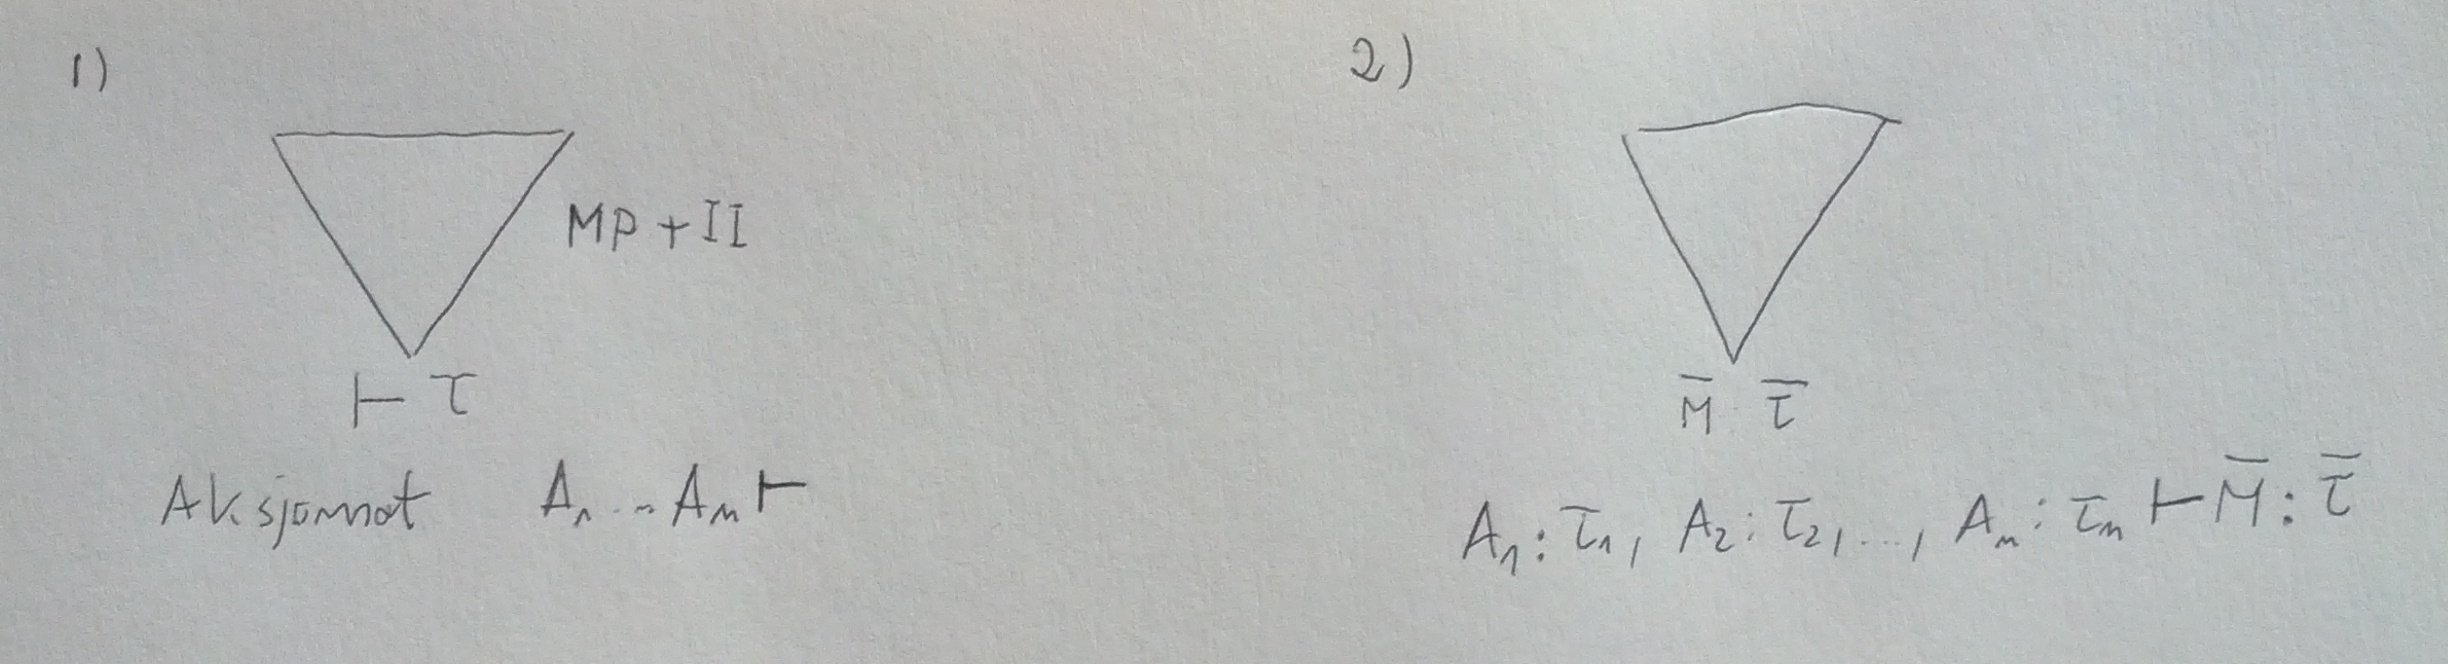
\includegraphics[width=0.8\textwidth]{img/typowaneWyprowadzenie}
\end{center}
Szukamy dowodów (w postaci termu $\lambda$)
\begin{align*}
\lambda x_A . x_A &: A \rightarrow A\\
\lambda x_A x_B . x_A &: A \rightarrow (B \rightarrow A)\\
\lambda x_{A\rightarrow (B\rightarrow C)} y_{A\rightarrow B} z_A
	.(x_{A\rightarrow (B\rightarrow C)}z_{A})(y_{A\rightarrow B}z_{A}) &:
	(A \rightarrow (B \rightarrow C))\rightarrow
		((A \rightarrow B) \rightarrow (A \rightarrow C)) \\
\lambda xyz . (xz)(yz) &\\
xyz . y(zx) 
	&: (A \rightarrow B) \rightarrow
		(( B \rightarrow C) \rightarrow ( A \rightarrow C)) \\
\\
((A\rightarrow A)\rightarrow A)\rightarrow A &\\
\lambda x_{(A\rightarrow A)\rightarrow A} . x (\lambda z_A . z_A) &\\
\lambda x_{(A \rightarrow A) \rightarrow A} . x (\lambda z_A . x(\lambda y_A)) & :
((A \rightarrow B)\rightarrow A) \rightarrow A \text{: nie ma programu}
\end{align*}
Rachunek $\lambda$-bez typów.
Dany jest term $\lambda$-rachunku M-domknięty.\\
Problem: Czy istnieje typ $\tau$ taki, że $\vdash M : \tau$.
\begin{definition}
$A$, $B$ - formuły (typy); $A$ jest bardziej ogólny niż $B$, gdy $B$ powstaje z $A$ przez podstawienie za zmienne w $A$ pewnych formuł.
\begin{center}
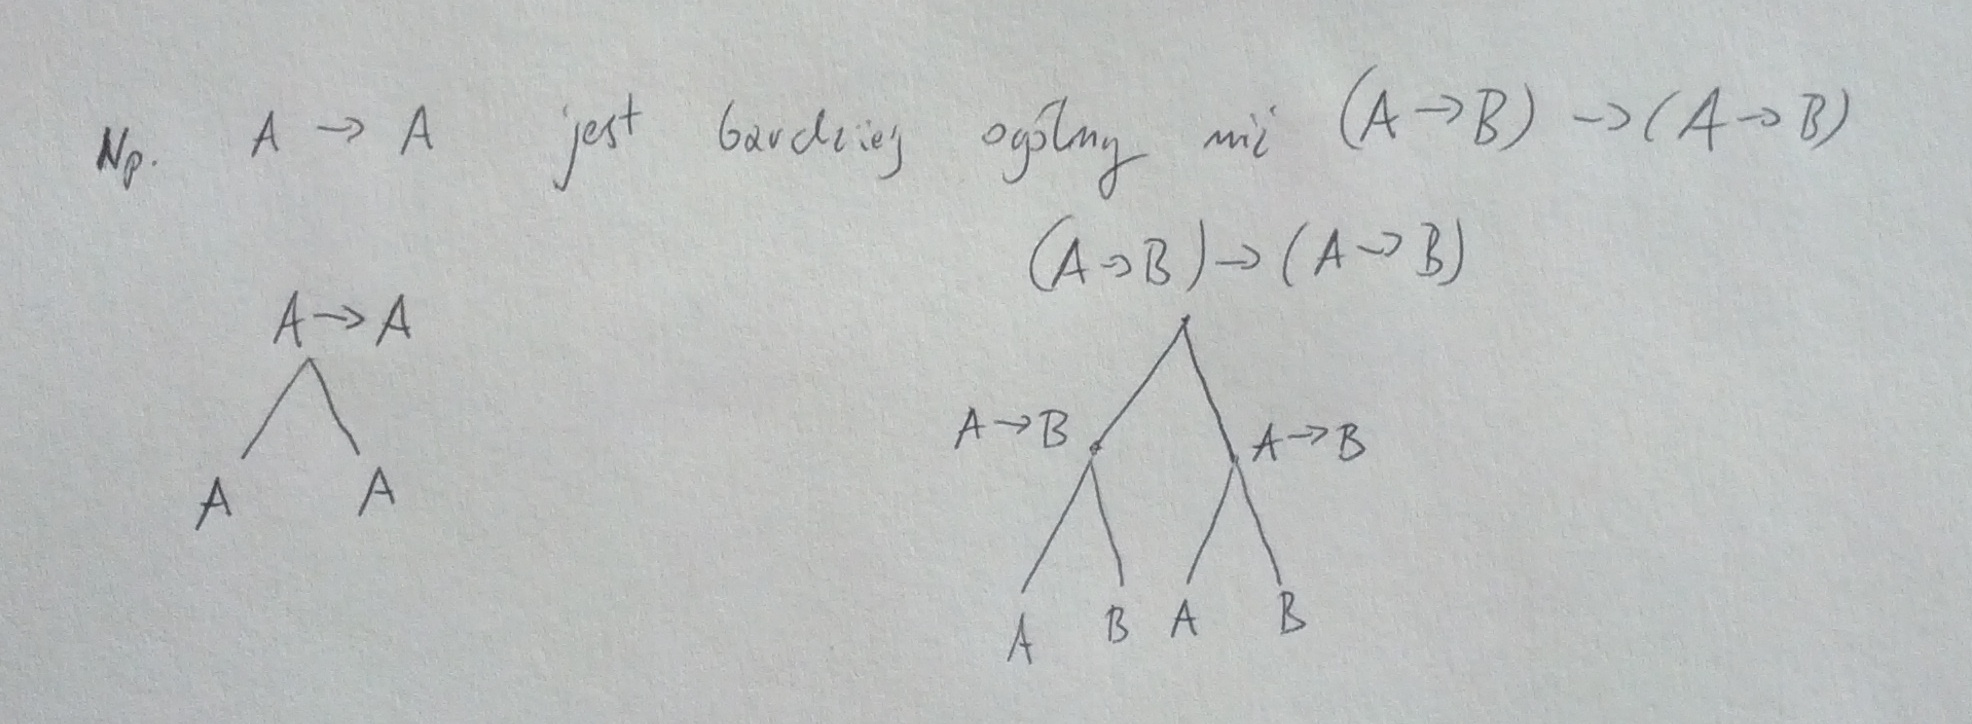
\includegraphics[width=0.8\textwidth]{img/podstawienieZmiennych}
\end{center}
Relacja ta jest przechodnia i zwrotna. $\leq$
\end{definition}

\begin{lemma}
$A \leq B$ i $B \leq A$ to $A$ i $B$ są identyczne z dokładnością do nazw zmiennych.
\end{lemma}


\begin{example}
$A \rightarrow (B \rightarrow A)$ jest identyczne z $C \rightarrow (B \rightarrow C)$
\end{example}

\begin{definition}
Term $M$-domknięty nietypowanego rachunku $\lambda$ jest typowany, gdy istnieje typ $\tau$ taki, że $\vdash M:\tau$
\end{definition}


\begin{theorem}[R. Hindley]
Istnieje algorytm mający na wejściu domknięty term $\lambda$ i zwracający najbardziej ogólny typ tego termu, o ile istnieje lub NIE, gdy nie istnieje.
\end{theorem}

\begin{theorem}[converse principal type algorithm]
Dla każdego typu $\tau$ takiego, że $\vdash \tau$ istnieje term $M$ taki, że $\vdash M:\tau$ i $\tau$ jest principal.
\end{theorem}

Przykłady znajdowania najbardziej ogólnego typu:
\begin{align*}
\underline{0} & = \lambda xy. y  & A \rightarrow (B \rightarrow B) &\\
\underline{1} & = \lambda xy. xy  & (B \rightarrow C) \rightarrow (B \rightarrow C) &\\
\underline{2} & = \lambda xy. x(xy) &  (B \rightarrow B) \rightarrow (B \rightarrow B) & \quad \mathbb{N} \text{ (typ liczb naturalnych)}
\end{align*}
Typ operacji arytmetycznych: $\mathbb{N} \rightarrow(\mathbb{N} \rightarrow\mathbb{N})$\\
Słowa: $(B\rightarrow B) \rightarrow ((B\rightarrow B) \rightarrow (B\rightarrow B))$\\
Drzewa: $(B\rightarrow B\rightarrow B) \rightarrow (B \rightarrow B)$\\
sklejanie drzew: $\textbf{(B$\rightarrow$ B$\rightarrow$ B)} \rightarrow (B \rightarrow B)$\\
początkowy węzeł: $(B\rightarrow B\rightarrow B) \rightarrow (\textbf{B} \rightarrow B)$\\
\\
$\lambda z_{B\rightarrow B\rightarrow B} x_B . z(zxx)(zx(zxx))$
\begin{center}
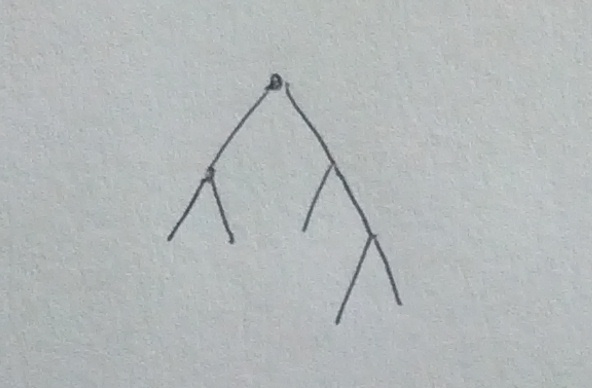
\includegraphics[width=0.3\textwidth]{img/lambdaTermJakoDrzewo}
\end{center}
Czy istnieje typ dla $\lambda x . xx$?\\
Jeśli typy są skończone to nie.\\
\\
Czy istnieje typ dla $\lambda xy . x(yx)$?
\begin{align*}
x &\text{ : } B\\
y &\text{ : } B \rightarrow C\\
x &\text{ : } C \rightarrow D
\end{align*}
$$(C\rightarrow D)\rightarrow((C\rightarrow D \rightarrow C)\rightarrow D)$$
Unknown headline.
\begin{center}
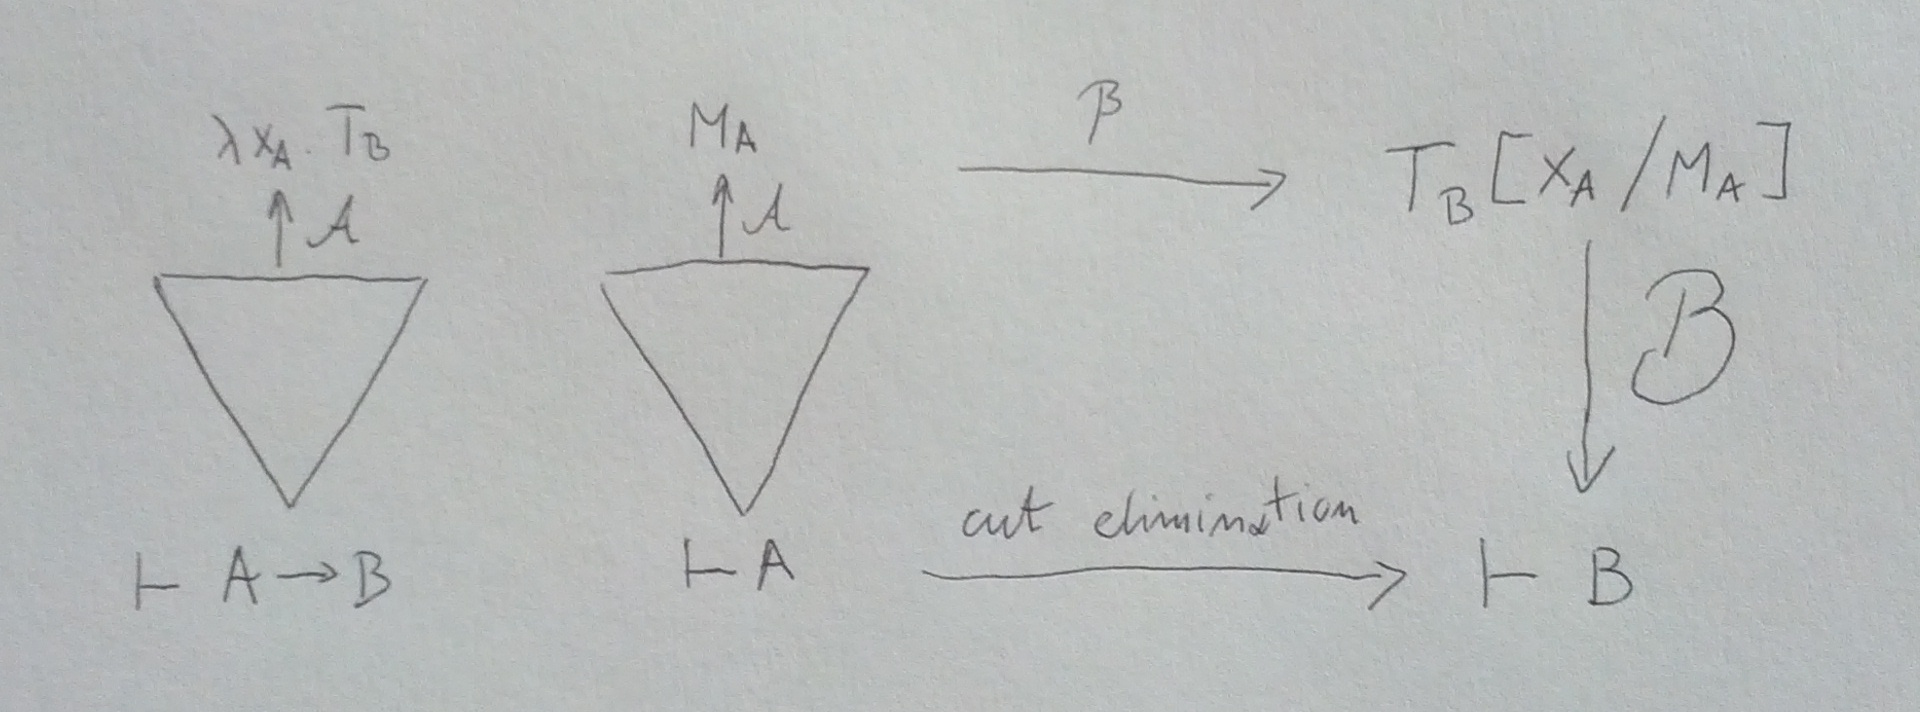
\includegraphics[width=0.8\textwidth]{img/rysunekWKtorymNieWiemOCoChodzi}
\end{center}

\section{Logika pierwszego rzędu}
\subsection{Oznaczenia}
\begin{itemize}
  \item Zmienne: $x, y, z,\ldots$
  \item Symbole funkcyjne (o~różnej arności): $f, g,\ldots$
  \item Symbole predykatywne (o~różnej arności): $p, q,\ldots$
  \item Stałe: $a,b,c,\ldots$ (można też na nie patrzeć jak na symbole funkcyjne
    o~arności 0).
\end{itemize}

\subsection{Definicje}
\begin{definition}[Term]
  ~\begin{itemize}
    \item Stałe i~zmienne są termami.
    \item Jeżeli $t_1,\ldots,t_k$ są termami, a~$f$ jest $k$-arnym symbolem
      funkcyjnym to $f(t_1,\ldots,t_k)$ też jest termem.
    \item Nic innego nie jest termem.
  \end{itemize}
\end{definition}

\begin{definition}[Formuła atomowa]
  \emph{Formuła atomowa} to napis $p(t_1,\ldots,t_n)$, gdzie $p$ jest $n$-arnym
  symbolem predykatywnym, a $t_1,\ldots,t_n$ -- termami.
\end{definition}

\begin{definition}[Literał]
  Literał to formuła atomowa bądź jej zaprzeczenie ($\lnot A$).
\end{definition}

\begin{definition}[Formuła]
  ~\begin{itemize}
    \item Formuła atomowa jest formułą.
    \item Jeśli $A$~i~$B$ są formułami i~$x$ zmienną to formułami są również:
    ,,$A\land B$'', ,,$A\lor B$'', ,,$A\impl B$'', ,,$\lnot A$'',
    ,,$A\leftrightarrow B$'', ,,$\forall x A$'' oraz ,,$\exists x A$''.
    \item Nic innego nie jest formułą.
  \end{itemize}
\end{definition}

\begin{definition}[Zmienna wolna, formuła domknięta]
  \emph{Zmienna wolna} to zmienna nieznajdująca się pod działaniem żadnego
  kwantyfikatora. \emph{Formuła domknięta} to taka formuła, która 
  nie ma żadnych zmiennych wolnych.
\end{definition}

\begin{definition}[Klauzula]
  \emph{Klauzula} to formuła postaci:
  \[
    \forall x_1 \forall x_2 \ldots \forall x_m
      L_1 \lor L_2 \lor \ldots \lor  L_n
  \]
  gdzie $L_1, L_2, \ldots, L_n$ to literały, a $\lbrace x_1, x_2, \ldots, x_m
  \rbrace$ jest zbiorem wszystkich zmiennych występujących
  w~$L_1, L_2,\ldots, L_n$.
\end{definition}

\begin{definition}[Notacja ze strzałką dla klauzul]
$A_1,\ldots,A_p \leftarrow B_1,\ldots,B_q$ oznacza klauzulę
$\forall x_1 \ldots \forall x_n
  A_1 \lor \ldots \lor A_p\lor
  \lnot B_1 \lor \ldots \lor \lnot B_q$.
\end{definition}

\begin{definition}[Szczególne klauzule]
  ~\begin{itemize}
    \item Klauzula programu: $A \leftarrow B_1,\ldots,B_q$ dla $q \ge 0$
    \item Fakt: $A \leftarrow$
    \item Sprzeczność: $\leftarrow$ (inne oznaczenie:~$\square$)
    \item Klauzula celu: $\leftarrow B_1,B_2,\ldots,B_q$
    \item Klauzula Horna: klauzula programu lub celu
  \end{itemize}
\end{definition}

\begin{definition}[Program]
  \emph{Program} to skończony zbiór klauzul programu.
\end{definition}

\section{Modele programów}
\subsection{Definicje}
\begin{definition}[Model]
  Model $M$ to para $(D, I)$, gdzie $D \ne \emptyset$ jest \emph{dziedziną},
  a~$I$ -- \emph{interpretacją symboliki}. 

  $I(a) \in D$, gdy $a$ jest stałą; $I(f) \in D^{D^n}$, gdy $f$ jest funkcją
  $n$-arną; $I(p) \in \lbrace 0, 1 \rbrace^{D^n}$, gdy $p$ jest predykatem
  $n$-arnym.
\end{definition}

\begin{definition}[Interpretacja termów i formuł]
  Ustalmy model $M=(D,I)$.  Niech $v$ będzie \emph{oceną zmiennych},
  czyli funkcją $v : \lbrace x, y, z,\ldots \rbrace \rightarrow D$.
  Wtedy $\text{val}^{M,v}(t)$ jest \emph{interpretacją termu} $t$:
  \begin{itemize}
    \item $\text{val}^{M,v}(x) = v(x)$ ($x$ -- zmienna)
    \item $\text{val}^{M,v}(a) = I(a)$ ($a$ -- stała)
    \item $\text{val}^{M,v}(f(t_1,t_2,\ldots,t_n)) =
      I(f)(\text{val}^{M,v}(t_1), \mathrm{val}^{M,v}(t_2), \ldots,
      \text{val}^{M,v}(t_n))$ ($f$ -- funkcja $n$-arna)
  \end{itemize}
  Natomiast $\text{val}^{M,v}(\Phi)$ jest \emph{interpretacją formuły} $\Phi$:
  \begin{itemize}
    \item $\text{val}^{M,v}(p(t_1,t_2,\ldots,t_n)) =
      I(p)(\text{val}^{M,v}(t_1), \mathrm{val}^{M,v}(t_2), \ldots,
      \text{val}^{M,v}(t_n))$ ($p$ -- predykat $n$-arny)
    \item $\text{val}^{M,v}(\phi \impl \psi) =
      \max(1 - \text{val}^{M,v}(\phi), \mathrm{val}^{M,v}(\psi))$
      ($\phi$, $\psi$ -- formuły)
    \item Pozostałe spójniki logiczne definiujemy analogicznie
    \item $\text{val}^{M,v}(\forall x \Psi) = \begin{cases}
        1 & \text{gdy istnieje } d \in D \text{ takie, że }
        \text{val}^{M,v'}(\Psi) = 1 \\
        0 & \text{wpp}
      \end{cases}$, gdzie $v'$ jest wartościowaniem $v$ z~$x$ podmienionym
      na $d$: $v'(\phi) = \begin{cases} v(\phi) & \text{gdy } \phi \ne x \\
      d & \text{gdy } \phi = x \end{cases}$
    \item $\text{val}^{M,v}(\exists x \Psi)$ definiujemy analogicznie
  \end{itemize}

  Zauważmy, że jeśli $\Phi$ jest formułą domkniętą, to jej interpretacja
  $\text{val}^{M,v}(\Phi)$ nie zależy od $v$ -- będziemy więc ją oznaczać
  jako $\text{val}^{M}(\Phi)$.
\end{definition}

\begin{definition}[Model dla formuły]
  Model $M=(D,I)$ jest \emph{modelem dla formuły domkniętej} $\Phi$ gdy
  $\text{val}^M(\Phi) = 1$.
  
  Model $M$ jest \emph{modelem dla zbioru} $S$ formuł domkniętych wtedy i~tylko wtedy,
  gdy jest modelem dla każdej formuły ze zbioru $S$.
\end{definition}

\begin{definition}[Tautologia]
  Formuła $\Phi$ jest \emph{tautologią} gdy każdy model $M$ jest modelem dla
  $\Phi$.
\end{definition} 

\begin{definition}[Formuła spełnialna]
  Formuła $\Phi$ jest \emph{spełnialna} gdy istnieje dla niej model.
\end{definition} 

\begin{definition}[Konsekwencja logiczna]
  Formuła $\Phi$ jest \emph{konsekwencją logiczną} zbioru formuł $S$
  gdy każdy model dla $S$ jest też modelem dla $\Phi$. Oznaczamy to następująco:
  $S \models \Phi$.

  \begin{theorem}
    $S \models \Phi$ wtedy i~tylko wtedy, gdy $S \cup \lbrace\lnot\Phi\rbrace$
    jest niespełnialny (dowód łatwy).
  \end{theorem}
\end{definition}

\subsection{Przykłady}
\subsubsection{Tautologie}
\begin{itemize}
  \item $\left(\exists y \forall x~p(x,y)\right) \impl \left(\forall x \exists
      y~p(x,y)\right)$
  \item $\left(\forall x~p(x, f(x)) \right) \impl \left(\forall x \exists 
    y~p(x,y)\right)$
\end{itemize}
\subsubsection{Paradoks fryzjera}
Fryzjer goli wszystkich tych, którzy nie golą się sami. Czy goli więc sam
siebie?  Łatwo zauważyć, że taki fryzjer nie może istnieć. Zapiszmy to 
za pomocą formuł. Niech $p(x)$ oznacza ,,$x$ jest fryzjerem'', a~$q(x, y)$ --
,,$x$ goli $y$''. Wtedy formuła stwierdzająca, że nie istnieje taki fryzjer
wygląda następująco:
\[
  \left[\forall x~p(x)\impl \forall y~\left(g(x,y) \leftrightarrow \lnot g(y,y)
  \right)\right] \impl \lnot \exists x~p(x)
\]

\subsubsection{Modele skończone i~nieskończone}
Wszystkie skończone modele są modelami dla tej formuły, ale istnieją modele
nieskończone (na przykład $(\mathbb{Z}, \lbrace p \text{ interpretujemy jako }\le
\rbrace)$), które nie są dla niej modelami:
\[
  \left[\left(\forall x~p(x,x)\right) \land \left(\forall x, y, z~\left(p(x,y)
    \land p(y,z)\right) \impl p(y,z)\right) \land \left(\forall x,y~p(x,y)\lor
  p(y,x)\right)\right] \impl \exists y \forall x~p(y,x)
\]
Interpretacja: ,,dla każdej symetrycznej, przechodniej i~pełnej relacji
istnieje element najmniejszy''.

\subsubsection{Program: dodawanie}
Stworzymy takie klauzule, żeby predykat $\text{ADD}(x,y,z)$ był spełniony tylko
dla $z = x+y$ (gdzie $x+1$ rozumiemy jako zastosowanie funkcji $s$ na $x$:
$s(x)$). Oprócz predykatu $\text{ADD}$ i~funkcji $s$ będzie nam jeszcze
potrzebna stała $0$.

\begin{center}\begin{tabular}{l | l | l}
  Nazwa & Postać ze strzałką & Postać standardowa \\
  \hline
  $C_1$ & $\text{ADD}(0, x, x) \leftarrow$ & $\forall x~\text{ADD}(0, x, x)$ \\
  $C_2$ & $\text{ADD}(s(x),y,s(z)) \leftarrow \text{ADD}(x,y,z)$ & 
    $\forall x, y, z~\left(\text{ADD}(s(x),y,s(z)) \lor \lnot \text{ADD}(x,y,z)
    \right)$ 
\end{tabular}\end{center}

\paragraph{Program dla $1 + 1 = 2$}\mbox{}\\

Dodajmy do klauzul $C_1$ i~$C_2$ klauzulę celu $G$:

\begin{center}\begin{tabular}{l | l | l}
  Nazwa & Postać ze strzałką & Postać standardowa \\
  \hline
  $G$ & $\leftarrow \text{ADD}(s(0), s(0), s(s(0)))$ & $\lnot \text{ADD}(s(0),
    s(0), s(s(0)))$ 
\end{tabular}\end{center}

Pokażemy, że zbiór $\lbrace C_1, C_2, G \rbrace$ jest niespełnialny, a~co za tym
idzie, że $\lbrace C_1, C_2 \rbrace \models$\linebreak
$\text{ADD}(s(0), s(0), s(s(0)))$.
\begin{proof}
  Załóżmy, że $\lbrace C_1, C_2, G \rbrace$ jest spełnialny. Do $C_2$
  podstawiamy $x := 0, y:= s(0), z:=s(0)$.
  \[
    \text{ADD}(s(0),s(0),s(s(0))) \lor \lnot \text{ADD}(0, s(0), s(0))
  \]
  Założyliśmy, że w~naszym modelu zachodzi $G$, więc:
  \[
    \lnot \text{ADD}(0, s(0), s(0))
  \]
  Ale to stoi w~sprzeczności z~$C_1$ z~podstawionym $x:=s(0)$.
\end{proof}

\paragraph{Program dla $1+v = 2$}\mbox{}\\

Dodajmy do klauzul $C_1$ i~$C_2$ klauzulę celu $G'$:

\begin{center}\begin{tabular}{l | l | l}
  Nazwa & Postać ze strzałką & Postać standardowa \\
  \hline
  $G'$ & $\leftarrow \text{ADD}(s(0), v, s(s(0)))$ &
    $\forall v~\lnot \text{ADD}(s(0), v, s(s(0)))$ 
\end{tabular}\end{center}

Pokażemy, że zbiór $\lbrace C_1, C_2, G' \rbrace$ jest niespełnialny, a~co za tym
idzie, że $\lbrace C_1, C_2 \rbrace \models$\linebreak
$\exists v~\text{ADD}(s(0), v, s(s(0)))$.

\begin{proof}
  Załóżmy, że $\lbrace C_1, C_2, G' \rbrace$ jest spełnialny.

\begin{center}
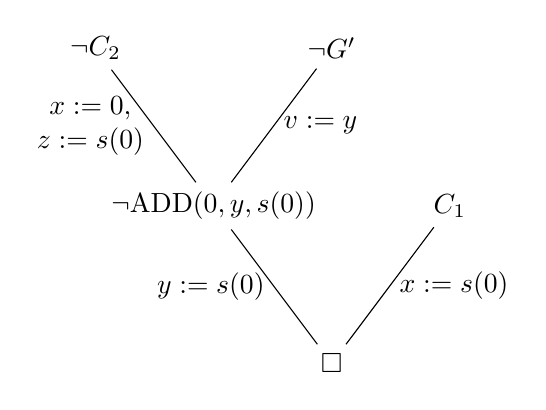
\begin{tikzpicture}[grow=up, level 1/.style={sibling distance=30mm},
  level distance=20mm]
  \node{$\square$}  
    child {
      node {$C_1$}
      edge from parent 
      node[right]{$x := s(0)$}
    }
    child {
      node {$\lnot\text{ADD}(0,y,s(0))$}
      child {
        node {$\lnot G'$}
        edge from parent 
        node[right]{$v := y$}
      }
      child {
        node {$\lnot C_2$}
        edge from parent 
        node[left, align=center]{$x := 0$,\\$z := s(0)$}
      }
      edge from parent 
      node[left]{$y := s(0)$}
    };
\end{tikzpicture}
\end{center}
\end{proof}

\end{document}
